%% PRE paper: EXTENDED METHODS AND RESULTS (internal checking document).
%% Detailed version of the main text + Supplemental Material: model and the
%% justification of each choice, every assumption and proof, and after each
%% result the numerical evidence (figures, numbers) and its analysis.
%% Math is shared with supplement.tex through math/*.tex (edit there only).
%% Compile: pdflatex pre_math_report && bibtex pre_math_report && pdflatex x2
\documentclass[11pt,a4paper]{article}
\usepackage[margin=2.2cm]{geometry}
\usepackage{amsmath,amssymb,amsthm,mathtools}
\usepackage{booktabs,longtable,array}
\usepackage{graphicx}
\usepackage{float}
\usepackage{xcolor}
\usepackage[font=small,labelfont=bf]{caption}
\usepackage[colorlinks=true,linkcolor=blue,citecolor=blue,urlcolor=blue]{hyperref}
\graphicspath{{../../figures/paper/}}

\newtheorem{proposition}{Proposition}
\newtheorem{lemma}[proposition]{Lemma}
\newtheorem{corollary}[proposition]{Corollary}
\theoremstyle{definition}
\newtheorem{definition}[proposition]{Definition}
\newtheorem{assumption}{Assumption}
\renewcommand{\theassumption}{A\arabic{assumption}}
\theoremstyle{remark}
\newtheorem{remark}[proposition]{Remark}
\newcommand{\E}{\mathbb{E}}
\newcommand{\Prob}{\mathbb{P}}
\newcommand{\avg}[1]{\langle #1\rangle}
\newcommand{\pend}[1]{\textcolor{red}{[Pending: #1]}}
\newenvironment{evidence}[1]{\subsection*{Numerical evidence and analysis: #1}%
  \addcontentsline{toc}{subsection}{Evidence: #1}}{}

\title{Targeted forcing of heterogeneous networks:\\ condensation, depletion and optimal targeting\\[4pt]
\large Extended methods and results for the PRE manuscript (internal)}
\author{Jose Herrera-Diestra}
\date{Working document, October 2026}

\begin{document}
\maketitle
\tableofcontents
\newpage

%%%%%%%%%%%%%%%%%%%%%%%%%%%%%%%%%%%%%%%%%%%%%%%%%%%%%%%%%%%%%%%%%%%%%%
\section{Question and summary of findings}
%%%%%%%%%%%%%%%%%%%%%%%%%%%%%%%%%%%%%%%%%%%%%%%%%%%%%%%%%%%%%%%%%%%%%%
\paragraph{Question.} An external process seeds a network repeatedly through a
subset of entry nodes. Each seeding event lands on entry node $i$ with
probability $\pi_i\propto w_i^\gamma$, where $w_i$ is a heterogeneous importance of the node
(its degree, in the epidemic application). How does the concentration of
forcing, $\gamma$, interact with the heterogeneity of $w$ to determine the total
cascade size? The dynamics are a stochastic SIR epidemic on a bipartite
network; the pathogen is hypothetical.

\paragraph{Findings} (each validated numerically; sections in brackets).
\begin{enumerate}
\item \textbf{Linear response.} One seeding event into a node of degree $k$ produces
$s(k)=Ak$ secondary cases below threshold, and the probability of none has a
closed form [\S\ref{sec:response}].
\item \textbf{Targeting gain.} The gain in secondary cases from targeting is
$\mu(\gamma)/\mu(0)$, independent of transmissibility and bounded by $k_{\max}/\mu(0)$. Near
threshold the absolute effect diverges but the relative effect does not
[\S\ref{sec:gain}].
\item \textbf{Depletion and $\gamma^*>0$.} Under repeated forcing, uniform targeting
maximizes the number of distinct entry nodes reached, but the burden is
maximized at a strictly positive $\gamma^*$. It is bounded by $\gamma_2$ only in the
large-population limit; finite pools under sparse forcing have $\gamma^*\ge\gamma_2$
[\S\ref{sec:depletion}, \S\ref{sec:optimal}].
\item \textbf{Targeting transition.} The targeting measure is a Gibbs measure. For
tails $p(w)\sim w^{-a}$ and responses $\propto w^\eta$, the targeted response diverges at
$\gamma_1=a-1-\eta$ and the forcing condenses at $\gamma_2=a-1$ [\S\ref{sec:transition}].
\item \textbf{Cut-off crossover.} A cut-off rounds the transition below
$n_c=(K_{\max}/k_0)^{a-1}/P_{\mathrm{tail}}$ and erases it above. Survey-calibrated networks lie
at $n/n_c\approx0.08$--$0.8$ [\S\ref{sec:transition}].
\item \textbf{Optimal targeting.} In the large-population limit $0<\gamma^*_\infty(x)\le\gamma_2$, with
$\gamma^*\simeq K/x$ for intense forcing and $\gamma_2-\gamma^*\simeq(a-1)/\ln(1/x)$ for sparse forcing.
Finite pools approach this limit from above, logarithmically in $n$
[\S\ref{sec:optimal}].
\item \textbf{Above threshold.} The probability of at least one major outbreak also
peaks at intermediate $\gamma$ [\S\ref{sec:threshold}].
\item \textbf{Illustration.} Survey-calibrated sexual networks are subcritical. With
a data-calibrated commercial-sex core, targeting decides whether a large
outbreak occurs [\S\ref{sec:illustration}].
\end{enumerate}

\paragraph{Scope of the degree model.} In the epidemic application the entry
nodes are class-1 nodes, so their degree law is the network's. Finite $A$ then
needs $a>3$. Results for $a=2.8$ apply only to the general importance model.

\paragraph{How to read this document.} Each section states the result with its
assumptions and proof (the same text as the Supplemental Material), followed
by a box ``Numerical evidence and analysis'' with the figures, the key
numbers, and an explanation of agreements, deviations and their meaning.

%% Notation table (report only).
%%%%%%%%%%%%%%%%%%%%%%%%%%%%%%%%%%%%%%%%%%%%%%%%%%%%%%%%%%%%%%%%%%%%%%
\section{Notation}
%%%%%%%%%%%%%%%%%%%%%%%%%%%%%%%%%%%%%%%%%%%%%%%%%%%%%%%%%%%%%%%%%%%%%%
\begin{longtable}{p{2.6cm}p{12.6cm}}
\toprule Symbol & Meaning \\ \midrule \endfirsthead
\toprule Symbol & Meaning \\ \midrule \endhead
$N_1,N_2$ & Sizes of the two node classes of the bipartite network (men, women) \\
$k$ & Degree; $p_k$, $q_k$ degree distributions of classes 1 and 2 \\
$\kappa_1,\kappa_2$ & Mean excess degrees $\avg{k(k-1)}/\avg{k}$ of classes 1 and 2 \\
$B$, $n=|B|$ & Set of entry nodes (bridges, a subset of class 1) and its size \\
$w_i$ & Importance of entry node $i$ (in the application $w_i=k_i$) \\
$a$ & Tail exponent: $f(w)\simeq C_0(a-1)w^{-a}$, $\Prob(W\ge w)\simeq C_0w^{-(a-1)}$ \\
$C_0$, $k_0$, $P_{\mathrm{tail}}$ & Tail amplitude; for a tail starting at $k_0$, $\Prob(W\ge w)=P_{\mathrm{tail}}(w/k_0)^{-(a-1)}$, $C_0=P_{\mathrm{tail}}k_0^{a-1}$ \\
$\gamma$ & Targeting exponent \\
$\pi_i(\gamma)$ & Targeting probability $w_i^\gamma/\sum_{j\in B}w_j^\gamma$ \\
$\ell_i$ & $\log w_i$ \\
$\alpha_t$ & Relative forcing intensity on day $t$, $\alpha_t\in[0,1]$ \\
$\beta_{\mathrm{ext}}$ & Forcing rate \\
$c$ & Expected number of seeding events without depletion, $\beta_{\mathrm{ext}}n\sum_t\alpha_t$ \\
$x$ & Seeding events per entry node, $c/n$ \\
$p$, $r$ & Daily transmission and recovery probabilities \\
$D$ & Number of transmission days of an infected node \\
$\tau$ & Per-edge transmissibility $\E[1-(1-p)^D]$ \\
$R$ & $\tau\sqrt{\kappa_1\kappa_2}$ \\
$A$ & Response per unit importance, $\tau(1+\tau\kappa_2)/(1-R^2)$ in the degree model \\
$\eta$ & Response exponent: a seeding event at $i$ causes $Aw_i^\eta$ secondary cases \\
$\mu_\eta(\gamma)$ & Targeted response $\sum_i\pi_iw_i^\eta$; $\mu\equiv\mu_1$ \\
$I(\gamma)$, $C(\gamma)$ & Expected realized seedings and expected total cascade size \\
$\gamma^*$ & $\arg\max_\gamma C(\gamma)$; $\gamma^*_\infty(x)$ its $n\to\infty$ limit at fixed $x$ \\
$\gamma_1^{(\eta)}$, $\gamma_2$ & $a-1-\eta$ and $a-1$ \\
$\theta_\eta(\gamma)$ & $d\log\mu_\eta/d\log n$ \\
$Y_2$ & Participation ratio $\sum_i\pi_i^2$ \\
$M(\gamma)$ & $\E[w^\gamma]$ \\
$\nu(\gamma)$ & $(a-1-\eta)/\gamma$ \\
$K$ & Large-$x$ constant, $\gamma^*\simeq K/x$ \\
$K_{\max}$, $n_c$ & Cut-off of $w$ and the crossover size $K_{\max}^{a-1}/C_0$ \\
\bottomrule
\end{longtable}



%%%%%%%%%%%%%%%%%%%%%%%%%%%%%%%%%%%%%%%%%%%%%%%%%%%%%%%%%%%%%%%%%%%%%%
%% MODEL
%%%%%%%%%%%%%%%%%%%%%%%%%%%%%%%%%%%%%%%%%%%%%%%%%%%%%%%%%%%%%%%%%%%%%%
%% Shared math (model); included by supplement.tex and pre_math_report.tex.
%%%%%%%%%%%%%%%%%%%%%%%%%%%%%%%%%%%%%%%%%%%%%%%%%%%%%%%%%%%%%%%%%%%%%%
\section{Model and assumptions}\label{sec:model}
%%%%%%%%%%%%%%%%%%%%%%%%%%%%%%%%%%%%%%%%%%%%%%%%%%%%%%%%%%%%%%%%%%%%%%

\begin{assumption}[network]\label{as:net}
The network is a static bipartite configuration model with degree
distributions $p_k$ (class 1) and $q_k$ (class 2), with finite second moments.
\end{assumption}
\begin{assumption}[tree-like]\label{as:tree}
Clusters started by finitely many seedings are locally tree-like: partners
reached from an infected node are distinct, previously susceptible, and have
numbers of other partners drawn independently from the excess-degree
distributions $p^{(1)}_j=(j+1)p_{j+1}/\avg{k}$ (and $q^{(1)}_j$).
\end{assumption}
\begin{assumption}[transmission]\label{as:sir}
Discrete days. Each infectious node infects each susceptible partner
independently with probability $p$ per day; then every infectious node,
including those infected that day, recovers with probability $r$. Runs
continue until extinction.
\end{assumption}
\begin{assumption}[entry nodes]\label{as:entry}
Entry nodes are a subset $B$ of class 1 chosen independently of degree, with
$k\ge1$. Their importances $w_i$ are i.i.d.
\end{assumption}
\begin{assumption}[forcing]\label{as:forcing}
On day $t\le T$ each susceptible entry node $i$ is seeded with probability
$1-\exp(-\beta_{\mathrm{ext}}\alpha_tn\pi_i)$, independently. A seeding aimed at a
non-susceptible node is lost (not redirected).
\end{assumption}
\begin{assumption}[independent clusters]\label{as:indep}
Clusters started by different seedings do not overlap, and entry nodes are
not infected through the network before they are seeded.
\end{assumption}
\begin{assumption}[tail]\label{as:tail}
$w$ has a regularly varying tail, $\Prob(W\ge w)\simeq C_0w^{-(a-1)}$, $a>1$; for
results involving $\eta$ we require $0<\eta<a-1$ (finite mean response). In the degree
model ($w=k$, entry-node degrees following the class-1 law) we also require
$a>3$, so that $\kappa_1$ and hence $A$ are finite.
\end{assumption}

\begin{remark}
\ref{as:tree} fails near the epidemic threshold and for small, densely shared
cores. The error of \ref{as:indep} is of the order of the attack fraction
$C/(N_1+N_2)$; it is largest when seeding is intense and transmissibility high.
The limit $n\to\infty$ at fixed $x$ keeps this fraction finite, so the asymptotic
results are statements about the allocation problem with overlaps neglected.
Both limitations are quantified numerically (Section~\ref{sec:validation}).
\end{remark}



\subsection*{Justification of the modelling choices}
\addcontentsline{toc}{subsection}{Justification of the modelling choices}
\begin{itemize}
\item \emph{Bipartite configuration model.} The application is transmission
through opposite-sex partnerships, which are bipartite. The configuration
model is the minimal ensemble that fixes the degree distributions and nothing
else. Every effect found is then attributable to degree heterogeneity and to
targeting, and the model admits exact branching-process calculations.
Clustering, assortativity and loops are deliberately absent (but see the core
network in \S\ref{sec:illustration}).
\item \emph{Static network.} Degrees are numbers of partners over a year, which
is longer than the forcing period (17 weeks) and the infectious period (two
weeks on average). A static network is the standard first approximation and
keeps the theory exact. Temporal partnerships are left for future work.
\item \emph{Discrete days.} Surveillance and forcing data are daily or weekly. The
discrete-time rules give an exact and simple distribution of transmission
days, $\Prob(D=d)=r(1-r)^d$, so simulation and theory correspond exactly, including
the correlation between the partnerships of one infectious node.
\item \emph{Targeting $\pi_i\propto w_i^\gamma$ with fixed total initial hazard.} A one-parameter
family spanning low-degree targeting ($\gamma<0$), uniform ($\gamma=0$) and hub targeting
($\gamma>0$). Because the total initial hazard is fixed, $\gamma$ changes where forcing goes
but not, initially, how much. The power form is the natural choice for
heterogeneous importance and produces the Gibbs-measure structure. In the
epidemic application nobody chooses $\gamma$. It measures how strongly external
contact increases with internal partners, as expected when sexual activity is
correlated across partnership types, and $\gamma^*$ is the worst-case allocation of
importations. For a seeding campaign $\gamma^*$ is the best allocation of seeds.
\item \emph{Lost, not redirected, seedings.} An external contact with a person
already infected or recovered produces no new infection and is not
redirected to someone else. This is what creates depletion and the finite
optimum.
\item \emph{Entry nodes independent of degree, with $k\ge1$.} The bridge property
(external contacts) is assumed independent of the number of internal
partners. Nodes with $k=0$ are excluded because they are not connected to the
network; an earlier version of the model included them and produced a
spurious targeting effect. Correlations between entry-node status and degree
are left for future work.
\item \emph{No latent period.} With runs continued to extinction, a latent period
only delays infections; it does not change cluster sizes for single seedings,
and under forcing it shifts timing only.
\end{itemize}

%%%%%%%%%%%%%%%%%%%%%%%%%%%%%%%%%%%%%%%%%%%%%%%%%%%%%%%%%%%%%%%%%%%%%%
%% RESPONSE
%%%%%%%%%%%%%%%%%%%%%%%%%%%%%%%%%%%%%%%%%%%%%%%%%%%%%%%%%%%%%%%%%%%%%%
%% Shared math (response); included by supplement.tex and pre_math_report.tex.
%%%%%%%%%%%%%%%%%%%%%%%%%%%%%%%%%%%%%%%%%%%%%%%%%%%%%%%%%%%%%%%%%%%%%%
\section{Response to one seeding event}\label{sec:response}
%%%%%%%%%%%%%%%%%%%%%%%%%%%%%%%%%%%%%%%%%%%%%%%%%%%%%%%%%%%%%%%%%%%%%%

\begin{lemma}[transmission days and transmissibility; uses \ref{as:sir}]
$\Prob(D=d)=r(1-r)^d$, $d\ge0$, and
\[
\tau=\E[1-(1-p)^D]=\frac{(1-r)p}{p+r-pr}\le1-r.
\]
\end{lemma}
\begin{proof}
A node becomes infectious on some day and faces recovery that same day, so
$\Prob(D=0)=r$; each further day it transmits once and then recovers with
probability $r$, so $\Prob(D=d)=(1-r)^dr$. Then
$1-\tau=\E[(1-p)^D]=\sum_dr[(1-r)(1-p)]^d=r/(1-(1-r)(1-p))=r/(p+r-pr)$, and
$\tau=1-r/(p+r-pr)=(1-r)p/(p+r-pr)$. As $p\to1$, $\tau\to1-r$.
\end{proof}

\begin{lemma}[no secondary case; uses \ref{as:sir}]
For a seeded node with $k$ susceptible partners,
$\Prob(\text{no secondary case})=\E[(1-p)^{kD}]=r/(1-(1-r)(1-p)^k)$.
\end{lemma}
\begin{proof}
$\sum_dr(1-r)^d(1-p)^{kd}=r/(1-(1-r)(1-p)^k)$. Note it differs from $(1-\tau)^k$
because the $k$ edges share the same $D$.
\end{proof}

\begin{proposition}[linear response; uses \ref{as:net}--\ref{as:sir}]\label{prop:linear}
If $R^2=\tau^2\kappa_1\kappa_2<1$, a seeding into a class-1 node of degree $k$ causes
on average $s(k)=Ak$ secondary cases, $A=\tau(1+\tau\kappa_2)/(1-R^2)$.
\end{proposition}
\begin{proof}
Let $W_2$ ($W_1$) be the mean cluster size, including the root, started by a
class-2 (class-1) node infected along an edge. By \ref{as:tree} it has $\kappa_2$
($\kappa_1$) further partners on average, each infected with probability $\tau$; by
linearity of expectation (correlations through $D$ do not affect means)
$W_2=1+\tau\kappa_2W_1$, $W_1=1+\tau\kappa_1W_2$. Hence $W_1=(1+\tau\kappa_1)/(1-R^2)$,
$W_2=(1+\tau\kappa_2)/(1-R^2)$, finite iff $R^2<1$. The seeded node infects $\tau k$
partners on average, each starting a cluster of mean $W_2$: $s(k)=\tau kW_2$.
\end{proof}

\begin{remark}[general response]
In general we write the mean response of node $i$ as $Aw_i^\eta$. The degree
model is $w=k$, $\eta=1$. Other values of $\eta$ represent nonlinear responses,
for example when importance and spreading capacity are different but
correlated attributes.
\end{remark}



\begin{evidence}{linear response}
Simulations seed single nodes of a given degree in survey-calibrated networks
(\S\ref{sec:illustration}) at $\tau\in\{0.2,0.4,0.6,0.8,0.9\}$, over 100 independent networks
per distribution with 30 seeding events per degree and network. Standard
errors are computed between networks.
\begin{figure}[H]
\centering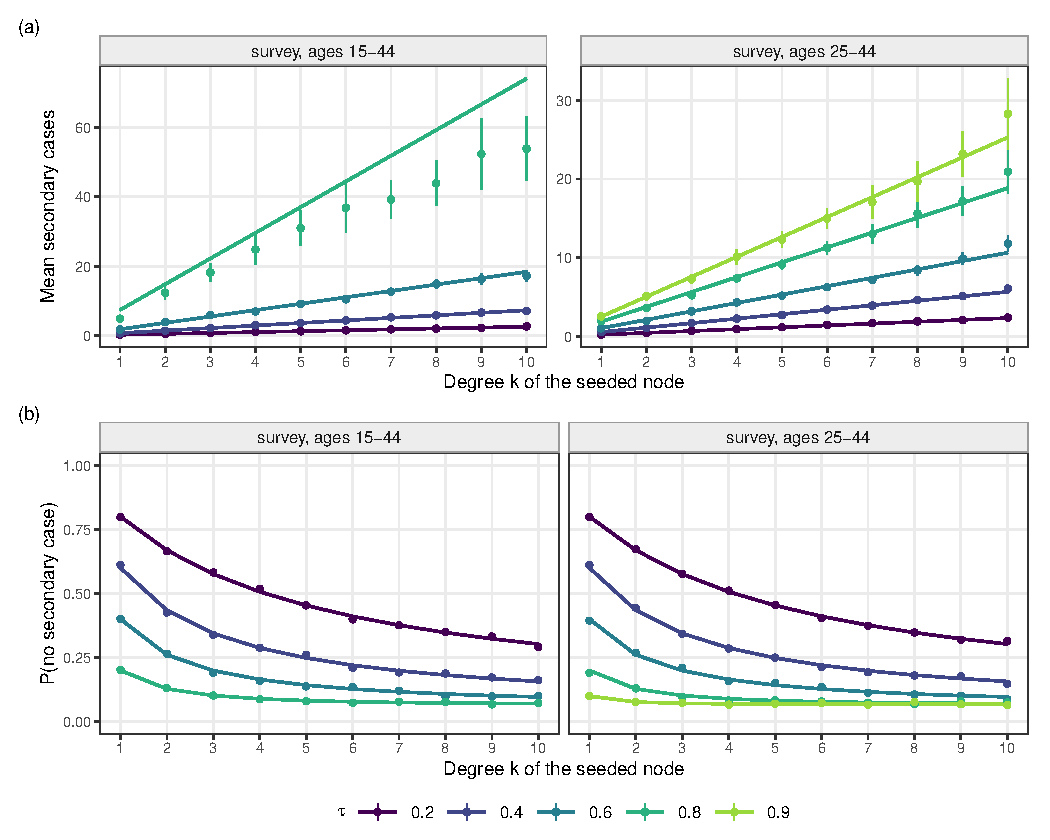
\includegraphics[width=\textwidth]{fig1_secondary_cases.pdf}
\caption{Linear response. (a) Mean secondary cases against the degree $k$ of the
seeded node (points: mean over 100 networks, $\pm2$ SE; degrees present in at least
five networks; lines: $s(k)=Ak$ with $\kappa$ from the pooled degree distribution).
(b) Probability of no secondary case (lines: $r/(1-(1-r)(1-p)^k)$).}
\label{fig:rep}
\end{figure}
\textbf{Numbers.} The median $|z|$ between simulation and $s(k)$ is below 1 for every
$\tau$ and both distributions, except ages 15--44 at $\tau=0.8$ ($R\approx0.94$), where the
simulation falls below the theory (for $k=1$: 4.9 against 7.4). The probability
of no secondary case agrees within 0.044 everywhere.

\textbf{Analysis.} (i) The probability of no secondary case depends only on the
seeded node's own partnerships and on $D$, so it is exact and matches
everywhere. It confirms the distribution of transmission days and the
correlation between partnerships (it differs from $(1-\tau)^k$). (ii) The mean
depends on the whole cluster and therefore on the tree-like approximation,
which fails near threshold, where clusters are large and loops and finite-size
depletion matter; the simulation then falls below the theory. The theory is
reliable for $R\lesssim0.9$. (iii) In a single network, rare degrees (one or a few
nodes) deviate because the neighbourhoods of those specific nodes differ from
the ensemble average. A node-level formula with the actual partners' degrees,
$s_i=\tau\sum_{j\in\mathcal N(i)}[1+\tau(k_j-1)M_\star]$, removes these deviations at $\tau\le0.4$. Averaging
over networks is the correct comparison for an ensemble result.
\end{evidence}

%%%%%%%%%%%%%%%%%%%%%%%%%%%%%%%%%%%%%%%%%%%%%%%%%%%%%%%%%%%%%%%%%%%%%%
%% GAIN
%%%%%%%%%%%%%%%%%%%%%%%%%%%%%%%%%%%%%%%%%%%%%%%%%%%%%%%%%%%%%%%%%%%%%%
%% Shared math (gain); included by supplement.tex and pre_math_report.tex.
%%%%%%%%%%%%%%%%%%%%%%%%%%%%%%%%%%%%%%%%%%%%%%%%%%%%%%%%%%%%%%%%%%%%%%
\section{Targeting gain per seeding event}\label{sec:gain}
%%%%%%%%%%%%%%%%%%%%%%%%%%%%%%%%%%%%%%%%%%%%%%%%%%%%%%%%%%%%%%%%%%%%%%

\begin{definition}
$\mu_\eta(\gamma)=\sum_{i\in B}\pi_i(\gamma)w_i^\eta$. Mean secondary cases per seeding:
$A\mu_\eta(\gamma)$; mean total per seeding: $1+A\mu_\eta(\gamma)$.
\end{definition}

\begin{proposition}\label{prop:gain}
(i) $G_{\mathrm{sec}}=\mu_\eta(\gamma)/\mu_\eta(0)$ does not depend on $A$ (hence not on
$\tau$, $\kappa_1$, $\kappa_2$). (ii) $d\mu_\eta/d\gamma=\mathrm{Cov}_\pi(\ell,w^\eta)\ge0$.
(iii) $G_{\mathrm{sec}}\to w_{\max}^\eta/\mu_\eta(0)$ as $\gamma\to\infty$.
(iv) $G_{\mathrm{tot}}=(1+A\mu_\eta(\gamma))/(1+A\mu_\eta(0))$ increases with $A$ when
$\mu_\eta(\gamma)>\mu_\eta(0)$ and tends to $G_{\mathrm{sec}}$ as $A\to\infty$ ($R\to1^-$).
\end{proposition}
\begin{proof}
(ii) $\pi_i=e^{\gamma\ell_i}/Z$ gives $d\pi_i/d\gamma=\pi_i(\ell_i-\bar\ell)$,
$\bar\ell=\sum_j\pi_j\ell_j$, so $d\mu_\eta/d\gamma=\sum_i\pi_i(\ell_i-\bar\ell)w_i^\eta=\mathrm{Cov}_\pi(\ell,w^\eta)$,
non-negative since $\ell$ and $w^\eta$ are increasing functions of $w$.
(iii) As $\gamma\to\infty$, $\pi$ concentrates on $\arg\max w$. (iv)
$\partial_AG_{\mathrm{tot}}=(\mu_\eta(\gamma)-\mu_\eta(0))/(1+A\mu_\eta(0))^2$.
\end{proof}



\begin{evidence}{targeting gain}
\begin{figure}[H]
\centering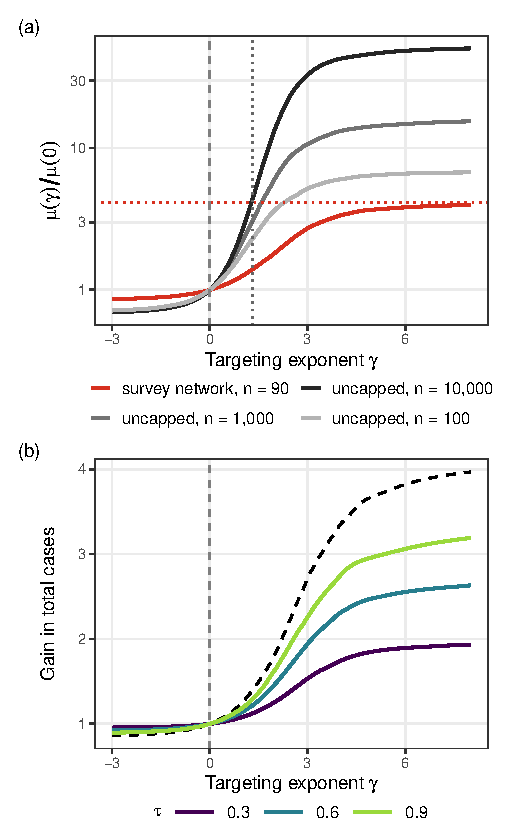
\includegraphics[width=\textwidth]{fig2_targeting_gain.pdf}
\caption{Targeting gain. (a) $\mu(\gamma)/\mu(0)$ for entry nodes of survey-calibrated
networks (red, median over 100 networks, degrees capped at 25; dotted: median
bound $k_{\max}/\mu(0)$) and for $n=10^2$, $10^3$, $10^4$ entry nodes drawn from the
uncapped survey law (grey, median over 200 samples). Dotted vertical line:
$\gamma_1=a-2=1.31$. (b) Gain in total cases on the survey networks for
$\tau\in\{0.3,0.6,0.9\}$; dashed: gain in secondary cases.}
\label{fig:gain}
\end{figure}
\textbf{Analysis.} The survey entry-node pool is nearly homogeneous (about 79 of
88 entry nodes have one partner; the maximum degree is 6--10), so the gain
saturates near $k_{\max}/\mu(0)\approx5$ and reaches it by $\gamma\approx4$. Uncapped pools of growing
size keep gaining beyond $\gamma_1$: the targeted degree grows with $n$, the first
sign of the transition of \S\ref{sec:transition}. In panel (b) the total gain
rises with $\tau$ towards the secondary-case gain, because the imported case
itself (the ``1'' in $1+A\mu$) weighs less when each importation is amplified more.
\end{evidence}

%%%%%%%%%%%%%%%%%%%%%%%%%%%%%%%%%%%%%%%%%%%%%%%%%%%%%%%%%%%%%%%%%%%%%%
%% DEPLETION
%%%%%%%%%%%%%%%%%%%%%%%%%%%%%%%%%%%%%%%%%%%%%%%%%%%%%%%%%%%%%%%%%%%%%%
%% Shared math (depletion); included by supplement.tex and pre_math_report.tex.
%%%%%%%%%%%%%%%%%%%%%%%%%%%%%%%%%%%%%%%%%%%%%%%%%%%%%%%%%%%%%%%%%%%%%%
\section{Repeated forcing and depletion}\label{sec:depletion}
%%%%%%%%%%%%%%%%%%%%%%%%%%%%%%%%%%%%%%%%%%%%%%%%%%%%%%%%%%%%%%%%%%%%%%

\begin{lemma}[uses \ref{as:forcing}, \ref{as:indep}]
Entry node $i$ is ever seeded with probability $1-e^{-c\pi_i}$.
\end{lemma}
\begin{proof}
While susceptible, it escapes day $t$ with probability $e^{-\beta_{\mathrm{ext}}\alpha_tn\pi_i}$,
independently across days; the product over $t\le T$ is
$e^{-\beta_{\mathrm{ext}}n\pi_i\sum_t\alpha_t}=e^{-c\pi_i}$. Under \ref{as:indep} nothing else
removes it from the susceptible pool before it is seeded.
\end{proof}

\begin{proposition}[depletion; uses \ref{as:net}--\ref{as:indep}]
\[
I(\gamma)=\sum_{i\in B}\left(1-e^{-c\pi_i}\right),\qquad
C(\gamma)=\sum_{i\in B}\left(1-e^{-c\pi_i}\right)\left(1+Aw_i^\eta\right).
\]
\end{proposition}

\begin{proposition}[optimal targeting is positive]\label{prop:pos}
Let $w$ not be constant on $B$. (i) $I(\gamma)\le I(0)$. (ii)
\[
\frac{dC}{d\gamma}=c\sum_i\pi_ie^{-c\pi_i}(\ell_i-\bar\ell)(1+Aw_i^\eta),\qquad
\left.\frac{dC}{d\gamma}\right|_0=c\,e^{-c/n}A\,\mathrm{Cov}_B(\ell,w^\eta)>0,
\]
with $\mathrm{Cov}_B$ the unweighted covariance over $B$. (iii) $C$ is non-decreasing on
$\gamma\le0$. (iv) Hence every maximizer satisfies $\gamma^*>0$, for all $c>0$. At finite $n$, $\gamma^*$
can be infinite when $c$ is small (the burden then increases up to complete
concentration); in the large-population limit it is finite
(Section~\ref{sec:optimal}). (v) $C(\gamma)=c(1+A\mu_\eta(\gamma))+O(c^2)$ as $c\to0$, non-decreasing in $\gamma$.
\end{proposition}
\begin{proof}
(i) Jensen: $\phi(\pi)=1-e^{-c\pi}$ is concave and $\sum\pi_i=1$, so
$\sum_i\phi(\pi_i)\le n\phi(1/n)=I(0)$. (ii) Differentiate and use
$d\pi_i/d\gamma=\pi_i(\ell_i-\bar\ell)$; at $\gamma=0$, $\pi_i=1/n$ and $\sum_i(\ell_i-\bar\ell)=0$
remove the constant 1. (iii) Write $dC/d\gamma=c\,\mathrm{Cov}_\pi(\ell,h)$ with
$h_i=e^{-c\pi_i}(1+Aw_i^\eta)$. For $\gamma\le0$, $\pi_i$ is non-increasing in $w_i$, so $e^{-c\pi_i}$ and
$1+Aw_i^\eta$ are non-decreasing in $w_i$, and so is $h$. The covariance of two
non-decreasing functions of $w$ is non-negative under any measure (Chebyshev's
sum inequality), so $dC/d\gamma\ge0$ on $\gamma\le0$. (iv) By (iii), $C(\gamma)\le C(0)$ for $\gamma<0$, and by
(ii), $C(\varepsilon)>C(0)$ for small $\varepsilon>0$. (v) Expand $1-e^{-c\pi}=c\pi+O(c^2)$ and use
Proposition~\ref{prop:gain}(ii).
\end{proof}



\begin{evidence}{depletion and the optimal exponent on networks}
Repeated forcing uses a 17-week incidence curve ($\sum_t\alpha_t=48.4$), with 50 networks
and 10 runs per combination of $c\in\{10,50,200\}$, $\tau\in\{0.6,0.9\}$ and $\gamma\in[-2,6]$. The
theory uses each network's own entry nodes and degrees.
\begin{figure}[H]
\centering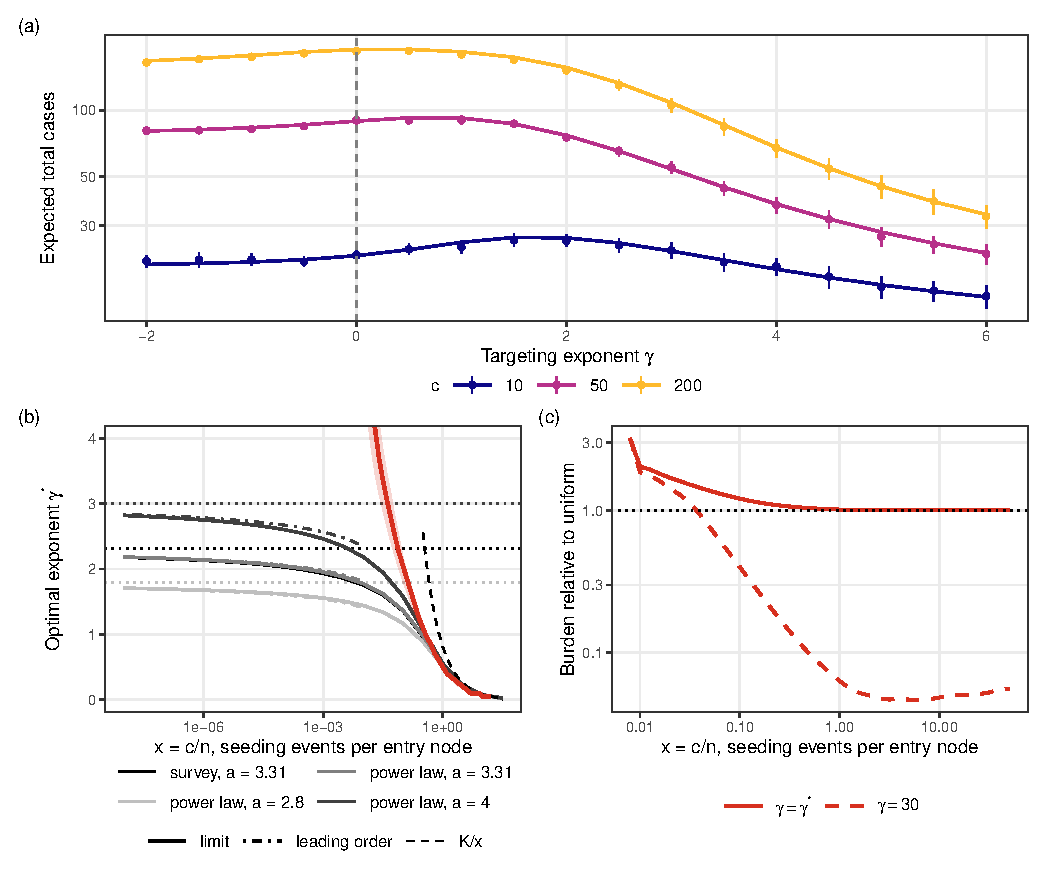
\includegraphics[width=\textwidth]{fig3_depletion_gamma_star.pdf}
\caption{Depletion. (a) Expected total cases against $\gamma$ ($\tau=0.6$; points:
simulation, $\pm2$ SE; lines: node-level theory). (b) $\gamma^*$ against $x=c/n$ for the
survey networks (red, median and IQR over 100 networks), the $n\to\infty$ limits for
uncapped laws (solid; $a=2.8$ only as an importance law), the leading order
$\gamma_2-(a-1)/\ln(1/x)$ (dot-dashed, $x\le10^{-2}$), $K/x$ for $A=2$ (dashed) and $\gamma_2$
(dotted). (c) Burden at $\gamma^*$ and at $\gamma=30$ relative to uniform targeting.}
\label{fig:dep}
\end{figure}
\textbf{Numbers.} Realized seedings: simulation and $I(\gamma)$ agree with $|z|<2$ in
every combination. Total cases: $|z|\lesssim2$, except $\tau=0.9$, $c=200$, where the
simulation is about 10\% below the theory. The overlap error scales with the
attack fraction $C/(N_1+N_2)$, which is largest in this combination. Optimum on networks: $\gamma^*\approx2$ ($c=10$),
0.5--1 ($c=50$), about 0.5 ($c=200$). Over 30\,960 combinations of network, $\tau$ and $c$ (script 04),
the exact derivative at $\gamma=0$ is positive in every case, every identifiable $\gamma^*$
is positive (smallest 0.05), and $\gamma=0$ maximizes $I$ in every case. The gain at $\gamma^*$
is 1.4--3.0 at $c=1$ and at most 1.02 for $c\ge100$. Extreme hub targeting lowers
the burden by a factor of about 10--20 at large $c$.

\textbf{Analysis.} $I(\gamma)$ depends only on the forcing and on which entry nodes are
still susceptible, so it is exact. Total cases add the cluster sizes and so
inherit the tree-like approximation and the assumption of non-overlapping
clusters. The 10\% shortfall under intense, highly transmissible forcing is the
expected overlap of clusters plus the infection of entry nodes through the
network before they are seeded. The trade-off is visible directly: moderate
concentration raises the burden because each seeding is amplified more, and
strong concentration lowers it because seedings are wasted on nodes already
reached. When forcing is sparse ($c\lesssim n$) amplification dominates up to large
$\gamma$; when it is intense almost every entry node is reached anyway, and
concentrating can only lose.
\end{evidence}

%%%%%%%%%%%%%%%%%%%%%%%%%%%%%%%%%%%%%%%%%%%%%%%%%%%%%%%%%%%%%%%%%%%%%%
%% TRANSITION
%%%%%%%%%%%%%%%%%%%%%%%%%%%%%%%%%%%%%%%%%%%%%%%%%%%%%%%%%%%%%%%%%%%%%%
%% Shared math (transition); included by supplement.tex and pre_math_report.tex.
%%%%%%%%%%%%%%%%%%%%%%%%%%%%%%%%%%%%%%%%%%%%%%%%%%%%%%%%%%%%%%%%%%%%%%
\section{The targeting transition}\label{sec:transition}
%%%%%%%%%%%%%%%%%%%%%%%%%%%%%%%%%%%%%%%%%%%%%%%%%%%%%%%%%%%%%%%%%%%%%%
$\pi_i=e^{\gamma\ell_i}/Z$ is a Gibbs measure with inverse temperature $\gamma$ and
energies $-\ell_i$ \cite{derrida1981random}. Throughout, \ref{as:entry} and
\ref{as:tail} hold and $n\to\infty$.

\begin{lemma}[tail index]
$w^s$ ($s>0$) has tail index $(a-1)/s$: $\Prob(W^s>y)\simeq C_0y^{-(a-1)/s}$. Hence
$\E[w^s]<\infty$ iff $s<a-1$, and $w_{\max}=\max_{i\le n}w_i\sim(C_0n)^{1/(a-1)}$.
\end{lemma}

\begin{proposition}[critical exponents]
$\gamma_1^{(\eta)}=a-1-\eta$ and $\gamma_2=a-1$, with
\[
\theta_\eta(\gamma)=\begin{cases}0,&\gamma<a-1-\eta,\\ \dfrac{\gamma-(a-1-\eta)}{a-1},&a-1-\eta<\gamma<a-1,\\[4pt] \dfrac{\eta}{a-1},&\gamma>a-1.\end{cases}
\]
\end{proposition}
\begin{proof}
$\mu_\eta=\overline{w^{\gamma+\eta}}/\overline{w^\gamma}$. If both exponents are below $a-1$, both
averages converge by the strong law of large numbers, whose converse
states that the empirical mean of nonnegative i.i.d.\ variables with infinite
expectation grows without bound \cite{durrett2019probability}. Hence $\theta=0$. If $\gamma+\eta>a-1>\gamma$, the denominator
converges and the numerator, a sum of i.i.d.\ variables with tail index
$(a-1)/(\gamma+\eta)<1$, is of the order of its maximum $w_{\max}^{\gamma+\eta}$, divided by
$n$: $\mu_\eta\sim n^{(\gamma+\eta)/(a-1)-1}$. If $\gamma>a-1$, both sums are of the order of
their maxima: $\mu_\eta\sim w_{\max}^{\gamma+\eta}/w_{\max}^{\gamma}=w_{\max}^\eta\sim n^{\eta/(a-1)}$.
\end{proof}

\begin{proposition}[condensation]
For $\gamma>\gamma_2$, the ranked targeting probabilities converge in law to
Poisson--Dirichlet $\mathrm{PD}(\beta_{\mathrm t},0)$ with $\beta_{\mathrm t}=(a-1)/\gamma<1$
\cite{pitman1997two}, and $\E[Y_2]\to1-(a-1)/\gamma$. For $\gamma<\gamma_2$, $Y_2\to0$.
\end{proposition}
\begin{proof}[Sketch]
Normalized i.i.d.\ positive weights with tail index $\beta_{\mathrm t}\in(0,1)$ converge to
$\mathrm{PD}(\beta_{\mathrm t},0)$; for this law $\E[\sum_iP_i^2]=1-\beta_{\mathrm t}$. For
$\beta_{\mathrm t}>1$ (finite mean), $Y_2\le\max_i\pi_i\to0$.
\end{proof}

\begin{remark}[finite-size scaling]
For finite $n$ the transition is rounded over a window of width $O(1/\log n)$
around $\gamma_2$; we test the scaling variable $(\gamma-\gamma_2)\log n$. In the condensed phase
$Y_2$ does not self-average.
\end{remark}

\begin{proposition}[cut-off crossover]
If $w\le K_{\max}$, all moments are finite and there is no transition as $n\to\infty$.
For finite $n$ the cut-off is irrelevant while $w_{\max}(n)\ll K_{\max}$, i.e.\ for
$n\ll n_c=K_{\max}^{a-1}/C_0=(K_{\max}/k_0)^{a-1}/P_{\mathrm{tail}}$, and dominates for $n\gg n_c$.
Capped/uncapped ratios of $\mu$ and $Y_2$ are therefore functions of $n/n_c$.
\end{proposition}
\begin{proof}
$w_{\max}$ solves $n\Prob(W\ge w_{\max})\approx1$, i.e.\ $nC_0w_{\max}^{-(a-1)}\approx1$. Setting
$w_{\max}=K_{\max}$ gives $n_c$.
\end{proof}



\begin{evidence}{the targeting transition}
Entry-node degrees are drawn i.i.d.\ without cap from pure power laws ($a=2.8$,
3.31, 4) and from the survey law with its power-law tail ($a=3.31$), and with a
cap of 25 for contrast; $n=10^2$ to $10^6$ (200--2000 samples per $n$).
\begin{figure}[H]
\centering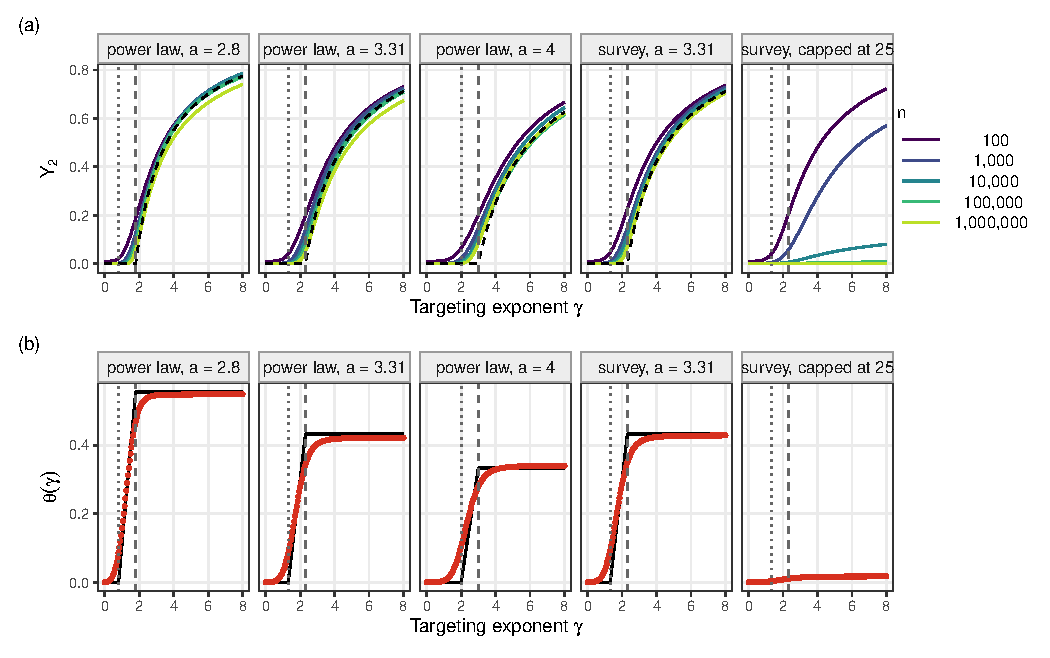
\includegraphics[width=\textwidth]{figS_transition.pdf}
\caption{Targeting transition for all laws (columns). (a) Participation ratio
$Y_2$ against $\gamma$ with the limit $1-(a-1)/\gamma$ (black dashed). (b) Fitted $\theta(\gamma)$
(points) against the piecewise prediction (lines). Vertical lines mark $\gamma_1$
(dotted) and $\gamma_2$ (dashed); in the capped column they mark the uncapped values.
The main text shows the survey column only.}
\label{fig:trans}
\end{figure}
\textbf{Numbers} ($n=10^6$). Plateau of $\theta$ (fit/theory): 0.548/0.556 ($a=2.8$),
0.422/0.433 (3.31), 0.339/0.333 (4), 0.428/0.433 (survey); capped law: 0.017.
$Y_2$ against its limit: 0.376/0.400 ($a=2.8$, $\gamma=3$), 0.269/0.250 ($a=4$, $\gamma=4$),
0.385/0.422 ($a=3.31$, $\gamma=4$), 0.606/0.615 (survey, $\gamma=6$).

\textbf{Analysis.} At finite $n$ the kinks of $\theta$ are rounded and the plateaus
are approached slowly. This is the expected logarithmic convergence near a
condensation point (the window shrinks as $1/\ln n$, which is what the collapse
below uses). Above $\gamma_2$, $Y_2$ does not self-average, so sample means fluctuate
by a few hundredths. The capped law shows neither transition, as predicted,
because all its moments are finite. Physically, $\ln w$ is exponentially
distributed with rate $a-1$, so $\pi$ is the equilibrium measure of Bouchaud's
trap model and $\gamma_2$ is its glass transition
\cite{bouchaud1992weak,bouchaud1995aging}.

\begin{figure}[H]
\centering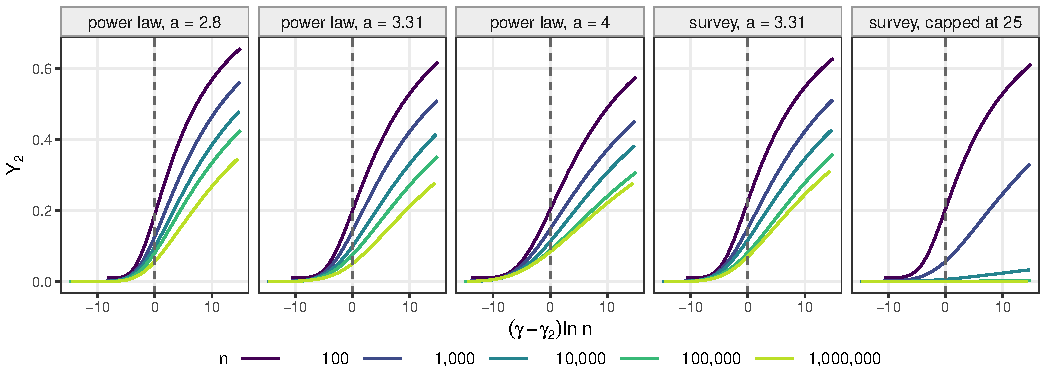
\includegraphics[width=\textwidth]{figS_scaling_Y2_collapse.pdf}\\[4pt]
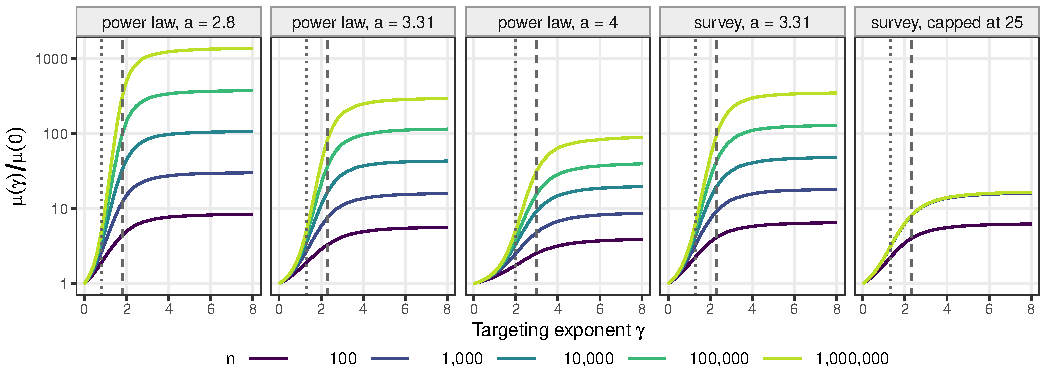
\includegraphics[width=\textwidth]{figS_scaling_mu.pdf}
\caption{Top: $Y_2$ against $(\gamma-\gamma_2)\ln n$; curves for different $n$ collapse.
Bottom: targeted mean degree $\mu(\gamma)/\mu(0)$ for $n=10^2$--$10^6$.}
\end{figure}

\paragraph{Generalization ($\eta\ne1$).}
\begin{figure}[H]
\centering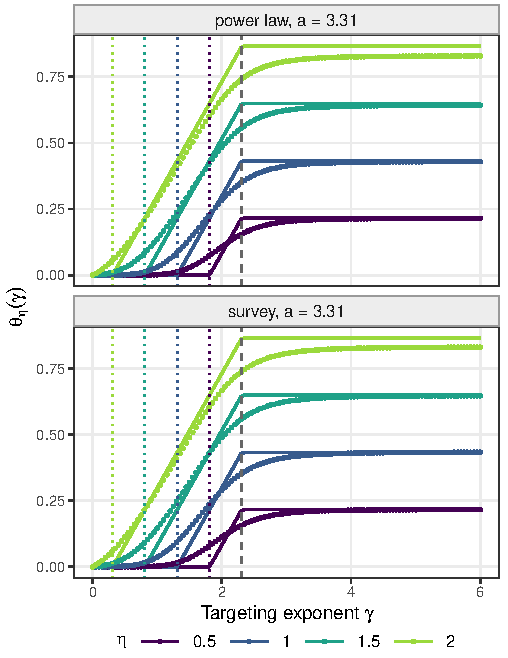
\includegraphics[width=\textwidth]{figS_gen_theta_eta.pdf}
\caption{$\theta_\eta(\gamma)$ for $\eta=0.5$, 1, 1.5, 2, power law $a=3.31$ (top) and survey law
(bottom). Points are fits over $n=10^3$--$10^6$, lines the prediction; dotted
lines $\gamma_1=a-1-\eta$, dashed line $\gamma_2$.}
\label{fig:theta_eta}
\end{figure}
The first kink moves with $\gamma_1=a-1-\eta$, and the plateaus are $\eta/(a-1)$: fit/theory
0.21/0.22, 0.43/0.43, 0.64/0.65 and 0.83/0.87 for $\eta=0.5$, 1, 1.5 and 2 (both laws).
The condensation point $\gamma_2$ does not move. Below $\gamma_2$ the prediction depends on $\gamma$
and $\eta$ only through $\gamma+\eta$, because only the numerator $\sum_iw_i^{\gamma+\eta}$ diverges there.
Finite-size rounding is largest for $\eta=2$ (fitted plateau 0.83 against 0.87),
consistent with the slow, logarithmic convergence near $\gamma_2$.

\paragraph{Cut-off crossover.}
\begin{figure}[H]
\centering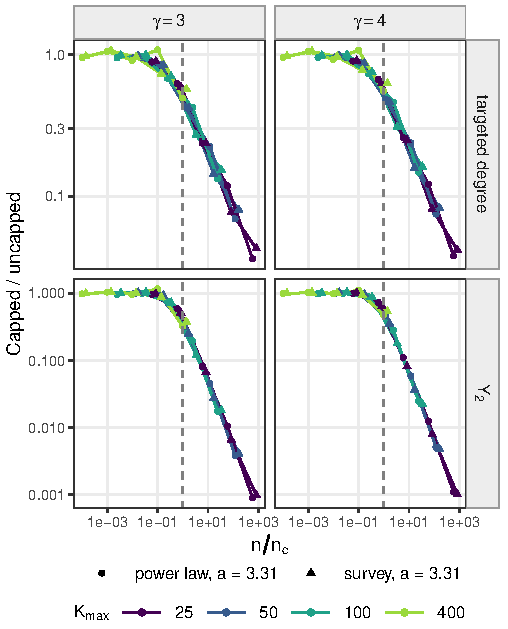
\includegraphics[width=0.9\textwidth]{figS_gen_crossover.pdf}
\caption{Capped/uncapped ratios of the targeted degree (top) and of $Y_2$ (bottom)
against $n/n_c$ for caps 25--400 and two laws, at $\gamma=3$ and 4. The dashed line
marks $n=n_c$.}
\label{fig:cross}
\end{figure}
All caps and both laws collapse onto one curve: ratios about 1 for $n/n_c\lesssim0.05$,
0.25--0.5 at $n/n_c\approx1$, and decaying beyond, since the uncapped quantities keep
growing with $n$ while the capped ones saturate. For the survey law with
$K_{\max}=25$, $n_c=(25/4)^{2.31}/0.0575\approx1.2\times10^3$. The entry-node pools of our networks
(about 90 and 940) sit at $n/n_c\approx0.08$ (transition fully visible) and $\approx0.8$ (in the
crossover).
\end{evidence}

%%%%%%%%%%%%%%%%%%%%%%%%%%%%%%%%%%%%%%%%%%%%%%%%%%%%%%%%%%%%%%%%%%%%%%
%% OPTIMAL TARGETING
%%%%%%%%%%%%%%%%%%%%%%%%%%%%%%%%%%%%%%%%%%%%%%%%%%%%%%%%%%%%%%%%%%%%%%
%% Shared math (optimal); included by supplement.tex and pre_math_report.tex.
%%%%%%%%%%%%%%%%%%%%%%%%%%%%%%%%%%%%%%%%%%%%%%%%%%%%%%%%%%%%%%%%%%%%%%
\section{Optimal targeting in the large-population limit}\label{sec:optimal}
%%%%%%%%%%%%%%%%%%%%%%%%%%%%%%%%%%%%%%%%%%%%%%%%%%%%%%%%%%%%%%%%%%%%%%

\begin{lemma}[limit burden; uses \ref{as:entry}, \ref{as:tail}]
At fixed $x=c/n$ and $\gamma<\gamma_2$,
\[
\frac{C(\gamma)}n\to\mathcal C(\gamma;x)=\E\!\left[\left(1-e^{-xw^\gamma/M(\gamma)}\right)\left(1+Aw^\eta\right)\right],
\qquad M(\gamma)=\E[w^\gamma].
\]
For $\gamma>\gamma_2$, $C/n\to0$. Hence $\gamma^*_\infty(x)\le\gamma_2$.
\end{lemma}
\begin{proof}
$c\pi_i=x\,w_i^\gamma/\overline{w^\gamma}$ and $\overline{w^\gamma}\to M(\gamma)<\infty$ (LLN), so
$C/n=\overline{(1-e^{-c\pi})(1+Aw^\eta)}\to\mathcal C$. For $\gamma>\gamma_2$ a finite share of the $xn$
seedings goes to $O(1)$ nodes, each seeded at most once, while the remaining
weights are $o(1)$ per node: the number of realized seedings is $o(n)$.
\end{proof}

\begin{proposition}[large-$x$ asymptote]
As $x\to\infty$, $\gamma^*\simeq K/x$, where $K>0$ is the unique root of
$g(K)=\E\!\left[(\ell-\avg{\ell})(1+Aw^\eta)\,w^{-K}\right]=0$.
\end{proposition}
\begin{proof}
First-order condition: $\sum_ie^{-xu_i}u_i(\ell_i-\bar\ell_\gamma)(1+Aw_i^\eta)=0$ with
$u_i=n\pi_i$. Put $\gamma=K/x$; then $u_i=1+\gamma d_i+O(\gamma^2)$, $d_i=\ell_i-\avg\ell$,
$\bar\ell_\gamma\to\avg\ell$, and $xu_i=x+Kd_i+O(K\gamma)$. Dividing by $e^{-x}$ and letting
$x\to\infty$: $\sum_ie^{-Kd_i}d_i(1+Aw_i^\eta)=0$, which is $g(K)=0$ up to the positive
factor $e^{K\avg\ell}$. Existence: $g(0)=A\,\mathrm{Cov}(\ell,w^\eta)>0$, and as $K\to\infty$ the
weight $w^{-K}$ concentrates on the smallest value $w_{\min}$, where $d<0$, so $g$
becomes negative. Uniqueness: with $d=\ell-\avg\ell$,
$g'(K)=-\E[d\,\ell\,(1+Aw^\eta)w^{-K}]=-\E[d^2(1+Aw^\eta)w^{-K}]-\avg\ell\,g(K)$, so at any root
$g'(K)=-\E[d^2(1+Aw^\eta)w^{-K}]<0$. Every root is a strict down-crossing of a
continuous function, hence there is only one.
\end{proof}

\begin{proposition}[small-$x$ asymptotics]\label{prop:smallx}
As $x\to0$, $\gamma^*_\infty(x)$ is asymptotically the interior local maximum, closest to
$\gamma_2$, of
\[
G(\gamma)=-\nu(\gamma)\left[\log\tfrac1x+\log M(\gamma)\right]+\log\Gamma\big(1-\nu(\gamma)\big),
\qquad \nu(\gamma)=\frac{a-1-\eta}{\gamma},
\]
which does not depend on $A$ or $C_0$. To leading order,
\[
\gamma_2-\gamma^*_\infty(x)\simeq\frac{a-1}{\log(1/x)}.
\]
\end{proposition}
\begin{proof}
Step 1. $\mathcal C=\E[1-e^{-xw^\gamma/M}]+A\,\E[(1-e^{-xw^\gamma/M})w^\eta]$. Since
$\E[xw^\gamma/M]=x$, the first term is $x-o(x)$ for every $\gamma$ and does not move the
maximum at leading order.\\
Step 2. In the second term, $\gamma+\eta>a-1$ on the interval considered, so the
expectation is dominated by $w$ near $w_s=(M/x)^{1/\gamma}\to\infty$, where the tail
density applies: $\E[(1-e^{-xw^\gamma/M})w^\eta]\simeq C_0(a-1)\int_0^\infty w^{\eta-a}(1-e^{-xw^\gamma/M})\,dw$.\\
Step 3. Substitute $u=xw^\gamma/M$: $w=(Mu/x)^{1/\gamma}$, $dw=\gamma^{-1}(M/x)^{1/\gamma}u^{1/\gamma-1}du$,
$w^{\eta-a}dw=\gamma^{-1}(M/x)^{(\eta-a+1)/\gamma}u^{-\nu-1}du$. The integral becomes
$\gamma^{-1}(x/M)^{\nu}\int_0^\infty u^{-\nu-1}(1-e^{-u})du$, convergent for $0<\nu<1$.\\
Step 4. Integration by parts: $\int_0^\infty u^{-\nu-1}(1-e^{-u})du=\nu^{-1}\Gamma(1-\nu)$. Since
$\gamma\nu=a-1-\eta$, $\mathcal C-x\simeq\frac{AC_0(a-1)}{a-1-\eta}(x/M)^\nu\Gamma(1-\nu)$; the prefactor
does not depend on $\gamma$, so maximizing $\mathcal C$ is maximizing $G=\log[(x/M)^\nu\Gamma(1-\nu)]$.\\
Step 5. Near $\gamma_2$, $M=m_0/\delta+O(1)$ with $\delta=\gamma_2-\gamma$, $m_0=C_0(a-1)$. Using
$d\nu/d\gamma=-\nu/\gamma$ and $d\log M/d\gamma\simeq1/\delta$, the stationarity condition $G'(\gamma)=0$
reads $(\nu/\gamma)[\log(1/x)+O(\log(1/\delta))]=\nu/\delta$, so $\delta\simeq\gamma/\log(1/x)\to\gamma_2/\log(1/x)$.
The terms of relative order $\log(1/\delta)/\log(1/x)$ are not all captured by $G$ (the
neglected $\gamma$-dependence of Step 1 and the regular part of $M$ enter at the same
order), so only the leading term is claimed.
\end{proof}

\begin{remark}[assumptions of Proposition~\ref{prop:smallx}]
(a) $0<\eta<a-1$; (b) $x\to0$ such that $w_s\to\infty$; (c) $\nu$ bounded away from 1,
i.e.\ $\gamma$ away from $\gamma_1^{(\eta)}$: as $\nu\to1$, $\log\Gamma(1-\nu)\to+\infty$ because the
integral of Step 3 is then dominated by small $w$, where the tail form does
not hold, so $G$ has a spurious divergence at $\gamma_1^{(\eta)}$ and the relevant
maximum is the interior one near $\gamma_2$; (d) Step 1 treats the $\gamma$-dependence of
the importation term as subleading.
\emph{Numerical check} (Section~\ref{sec:validation}): the leading order
matches the exact limit to within about 0.07 for $\eta\ge1$ and $x\le10^{-4}$ (e.g.\
$a=3.31$, $\eta=1$: 2.184 exact against 2.185 at $x=10^{-8}$), and converges more slowly
for $\eta=0.5$, where $\nu$ is close to 1 even near $\gamma_2$. The interior maximum of $G$
exists only below an $(a,\eta)$-dependent value of $x$; where it exists it
reproduces the exact limit to within $10^{-3}$--$10^{-6}$, so $G$ also captures the
subleading corrections numerically.
\end{remark}

\paragraph{Phase diagram of $\gamma^*$.} $0<\gamma^*_\infty(x)\le\gamma_2$ for all $x$ (positivity:
Proposition~\ref{prop:pos} applied to $\mathcal C$; the bound: the Lemma above; strict
inequality observed numerically; this bound holds only as $n\to\infty$); $\gamma^*_\infty\simeq K/x$ as
$x\to\infty$; $\gamma_2-\gamma^*_\infty\simeq(a-1)/\log(1/x)$ as $x\to0$. Finite $n$ approaches the limit from
above and only logarithmically in $n$ (numerics). For the survey law at $x=10^{-4}$,
$\gamma^*=5.95$ ($n=10^4$) and 2.45 ($n=10^6$), against $\gamma^*_\infty=2.03$ and $\gamma_2=2.31$; at $x=1$,
$\gamma^*=0.55$ already for $n=100$, against 0.52. The finite-$n$ optimum stays within 0.1 of
the limit only for $x\gtrsim3/\sqrt n$ over $n=10^2$--$10^6$.



\begin{evidence}{asymptotics of $\gamma^*$}
\begin{figure}[H]
\centering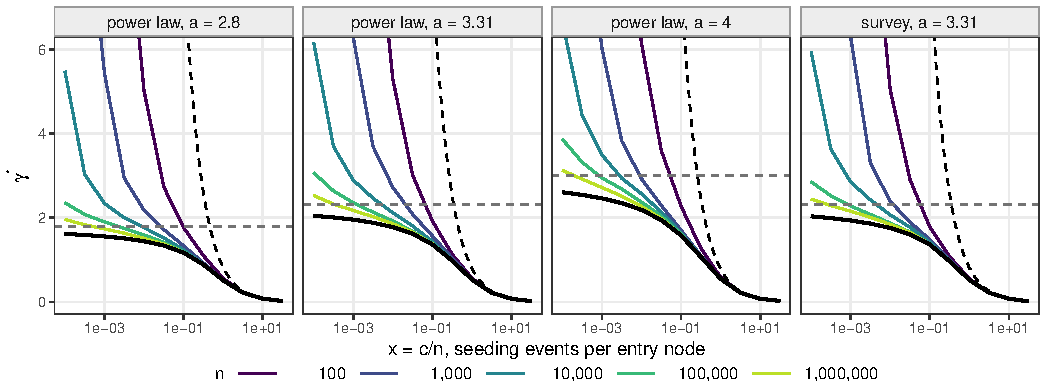
\includegraphics[width=\textwidth]{figS_scaling_gamma_star_limit.pdf}
\caption{$\gamma^*$ against $x$ for finite $n$ (colours, $A=2$), the exact $n\to\infty$ limit
(black), $K/x$ (dashed) and $\gamma_2$ (grey).}
\label{fig:gstar_lim}
\end{figure}
\begin{figure}[H]
\centering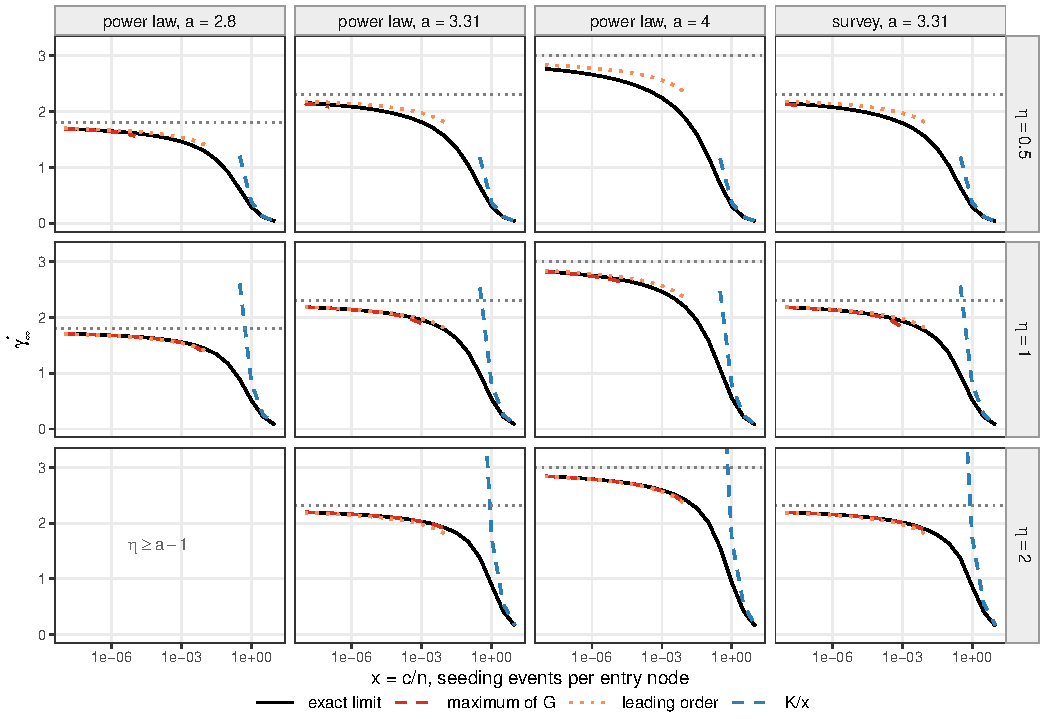
\includegraphics[width=\textwidth]{figS_gen_gamma_star_eta.pdf}
\caption{Exact limit (black) against the maximum of $G$ (red dashed, where its
interior maximum exists), the leading order $\gamma_2-(a-1)/\ln(1/x)$ (dotted,
$x\le10^{-2}$) and $K/x$ (blue dashed, $x\ge0.3$), for $\eta=0.5$, 1 and 2. The panel
$a=2.8$, $\eta=2$ is empty because $\eta\ge a-1$.}
\label{fig:gstar_eta}
\end{figure}
\begin{table}[H]
\centering\small
\caption{$K$ and the small-$x$ regime: exact limit / leading order / maximum of $G$
(``--'': no interior maximum, asymptotic regime not reached).}
\begin{tabular}{lccccc}
\toprule
Law & $a$ & $\eta$ & $K$ & $x=10^{-8}$ & $x=10^{-4}$ \\
\midrule
power & 2.80 & 0.5 & 0.380 & 1.694 / 1.702 / 1.693 & 1.558 / 1.605 / -- \\
power & 2.80 & 1 & 0.822 & 1.708 / 1.702 / 1.708 & 1.618 / 1.605 / 1.616 \\
power & 3.31 & 0.5 & 0.372 & 2.156 / 2.185 / 2.145 & 1.950 / 2.059 / -- \\
power & 3.31 & 1 & 0.799 & 2.184 / 2.185 / 2.184 & 2.048 / 2.059 / 2.036 \\
power & 3.31 & 2 & 1.734 & 2.195 / 2.185 / 2.195 & 2.092 / 2.059 / 2.091 \\
power & 4.00 & 0.5 & 0.365 & 2.768 / 2.837 / -- & 2.453 / 2.674 / -- \\
power & 4.00 & 1 & 0.779 & 2.820 / 2.837 / 2.818 & 2.607 / 2.674 / -- \\
power & 4.00 & 2 & 1.691 & 2.841 / 2.837 / 2.840 & 2.686 / 2.674 / 2.683 \\
survey & 3.31 & 0.5 & 0.375 & 2.152 / 2.185 / 2.138 & 1.936 / 2.059 / -- \\
survey & 3.31 & 1 & 0.810 & 2.181 / 2.185 / 2.181 & 2.034 / 2.059 / 2.018 \\
survey & 3.31 & 2 & 1.758 & 2.192 / 2.185 / 2.192 & 2.082 / 2.059 / 2.081 \\
\bottomrule
\end{tabular}
\end{table}
\textbf{Analysis.} (i) Finite $n$ approaches the limit from above, because small
pools cannot condense and so tolerate more concentration. Convergence is
logarithmic in $n$. At $x=10^{-4}$ (survey law), $\gamma^*=5.95$ for $n=10^4$ and 2.45 for
$n=10^6$, against $\gamma^*_\infty=2.03$ and $\gamma_2=2.31$. The finite-$n$ optimum is within 0.1 of
the limit only for $x\gtrsim3/\sqrt n$; at $x=1$ this holds already for $n=100$ (0.55
against 0.52). (ii) $K/x$ is accurate
for $x\gtrsim10$, within about 5\% (at $x=10$: 0.082, 0.080, 0.173 against the exact 0.078,
0.076, 0.157, for $a=2.8$, $\eta=1$; $a=3.31$, $\eta=1$; $a=3.31$, $\eta=2$), and
for $A=2$, $K$ depends mainly on $\eta$ ($\approx0.37$, 0.8, 1.7) and only weakly on $a$. $K$
also depends on $A$ and vanishes as $A\to0$, where uniform targeting is optimal. (iii) The leading
order captures the logarithmic approach to $\gamma_2$. It is within about 0.07 for
$\eta\ge1$ and $x\le10^{-4}$, and slower for $\eta=0.5$, because $\nu$ is then close to 1 even near
$\gamma_2$ and the tail approximation applies only at very small $x$. (iv) Where its
interior maximum exists, maximizing $G$ reproduces the exact limit to within
$10^{-3}$--$10^{-6}$; it contains the subleading corrections that the closed-form
leading order lacks. An earlier explicit next-order formula over-corrected and
is not used.
\end{evidence}

%%%%%%%%%%%%%%%%%%%%%%%%%%%%%%%%%%%%%%%%%%%%%%%%%%%%%%%%%%%%%%%%%%%%%%
%% ABOVE THRESHOLD
%%%%%%%%%%%%%%%%%%%%%%%%%%%%%%%%%%%%%%%%%%%%%%%%%%%%%%%%%%%%%%%%%%%%%%
%% Shared math (threshold); included by supplement.tex and pre_math_report.tex.
%%%%%%%%%%%%%%%%%%%%%%%%%%%%%%%%%%%%%%%%%%%%%%%%%%%%%%%%%%%%%%%%%%%%%%
\section{Above threshold}\label{sec:threshold}
%%%%%%%%%%%%%%%%%%%%%%%%%%%%%%%%%%%%%%%%%%%%%%%%%%%%%%%%%%%%%%%%%%%%%%
With $h(j,y)=\E_D[(1-\tau_D(1-y))^j]$, $\tau_D=1-(1-p)^D$, and $(u_1,u_2)$ the smallest
solution of $u_1=\sum_jp^{(1)}_jh(j,u_2)$, $u_2=\sum_jq^{(1)}_jh(j,u_1)$, a seeding into a class-1
node of degree $k$ starts a major outbreak with probability $1-h(k,u_2)$, and
$\Prob(\ge1\text{ major outbreak})=1-\prod_{i\in B}[e^{-c\pi_i}+(1-e^{-c\pi_i})h(k_i,u_2)]$. This
probability also peaks at intermediate $\gamma$ (numerics).



\begin{evidence}{major outbreaks}
Survey-calibrated networks cannot be pushed above threshold
(\S\ref{sec:illustration}), so this result is validated on synthetic
negative-binomial networks NB$(1.2,0.7)$ ($\kappa\approx3$, $\tau_c\approx0.33$). A run is major once
it reaches half the theoretical size of a major outbreak (minimum 100 cases).
\begin{figure}[H]
\centering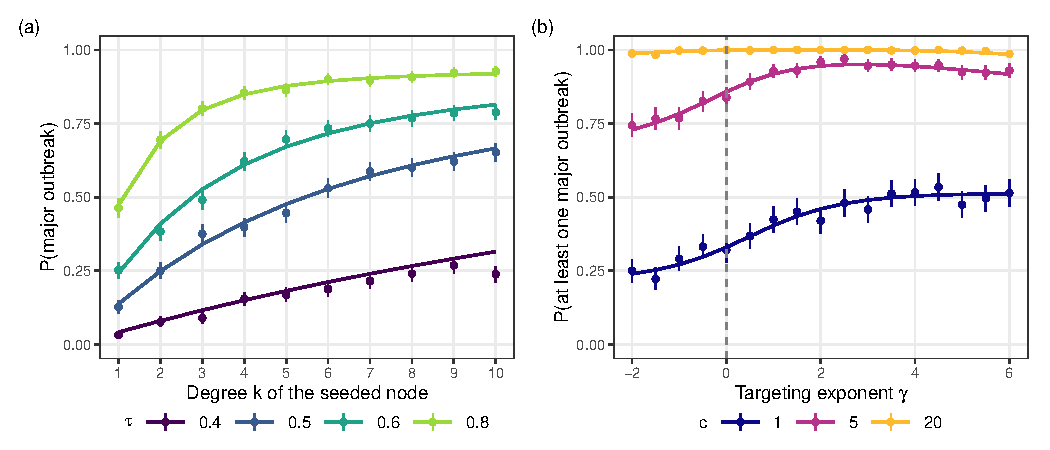
\includegraphics[width=\textwidth]{fig4_major_outbreaks.pdf}
\caption{(a) Probability that one seeding event into a node of degree $k$ starts a
major outbreak (20 networks $\times$ 50 events; lines: $1-h(k,u_2)$). (b) Probability of
at least one major outbreak under repeated forcing against $\gamma$.}
\end{figure}
\textbf{Numbers and analysis.} $|z|<2.3$ for $\tau\ge0.5$. At $\tau=0.4$ ($R\approx1.13$) the
simulation lies slightly below the theory, a finite-size effect close to
threshold. A first version used a fixed cut-off of 1000 cases, larger than the
major outbreaks near threshold, and misclassified them. The probability of at
least one major outbreak peaks at intermediate $\gamma$ (for $c=5$: 0.82 at $\gamma=0$, 0.95
at $\gamma=3$, 0.92 at $\gamma=6$). It is the same trade-off as for the burden, now acting on
the probability that some seeding event ignites a major outbreak.
\end{evidence}

%%%%%%%%%%%%%%%%%%%%%%%%%%%%%%%%%%%%%%%%%%%%%%%%%%%%%%%%%%%%%%%%%%%%%%
\section{Illustration: survey-calibrated sexual contact networks}\label{sec:illustration}
%%%%%%%%%%%%%%%%%%%%%%%%%%%%%%%%%%%%%%%%%%%%%%%%%%%%%%%%%%%%%%%%%%%%%%
\paragraph{Construction.} Degrees are numbers of opposite-sex partners in the
past year from the 2006--2008 NSFG \cite{chandra2011sexual} (ages 25--44: men
8.7/76.1/7.1/2.9/5.2\% with 0/1/2/3/4+ partners, women 8.2/82.7/5.4/1.7/1.9\%).
The 4+ class is spread over $k=4,\dots,25$ as $k^{-(\alpha+1)}$, with $\alpha=2.31$ (men) and 2.54
(women) \cite{liljeros2001web}; $\alpha$ is the exponent of a cumulative
distribution, hence the $+1$. Men's reporting excess is removed from men with
at least two partners (at most $k-1$ stubs each, in proportion to $k-1$). Women
and men without partners are then reproduced exactly, while men's share with
one partner rises from 76\% to 80\%. Entry nodes are bisexual men (probability
0.02 \cite{copen2016sexual}) with $k\ge1$: about 90 per $5\times10^3$ men, most with
one partner.

\paragraph{Properties.} Over 100 networks, $\kappa_1\in[0.51,0.82]$, $\kappa_2\in[0.54,1.07]$ and
$\sqrt{\kappa_1\kappa_2}\le0.92$, so the networks are subcritical at every attainable $\tau$ ($\tau\le0.931$).
Every seeding event produces a finite cluster, which is why the
below-threshold results apply directly.

\begin{figure}[H]
\centering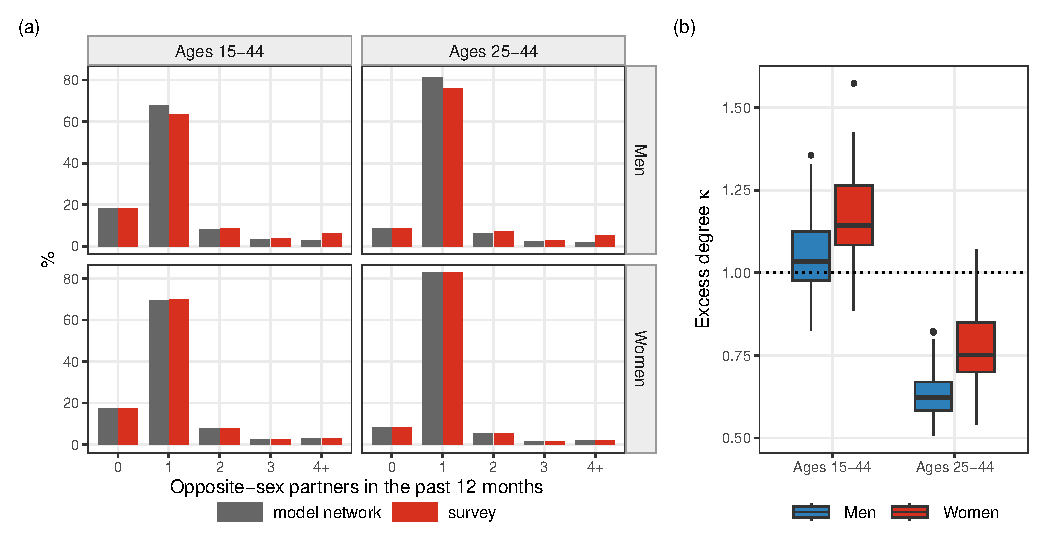
\includegraphics[width=0.85\textwidth]{figS1_network_calibration.pdf}
\caption{Survey calibration (a) and excess degrees across 100 networks (b).}
\end{figure}

\paragraph{Commercial-sex core.} Brewer et al.\ \cite{brewer2000prostitution}
showed that the men--women gap in reported partners is accounted for by sex
workers missing from household surveys. We therefore close the network by
assigning men's surplus to sex-worker nodes ($0.05\%$ of women, the measured
prevalence), with log-normal weights matching the reported median and mean.
Clients are chosen with weight $(k-1)^q$, $q=8$, so about 4.6\% of men are clients
(the floor compatible with the survey is 4.3\%). The implied number of partners
per sex worker (mean 240--360 per year) agrees with the independently measured
values. The core makes the network supercritical through a few hubs.

\begin{figure}[H]
\centering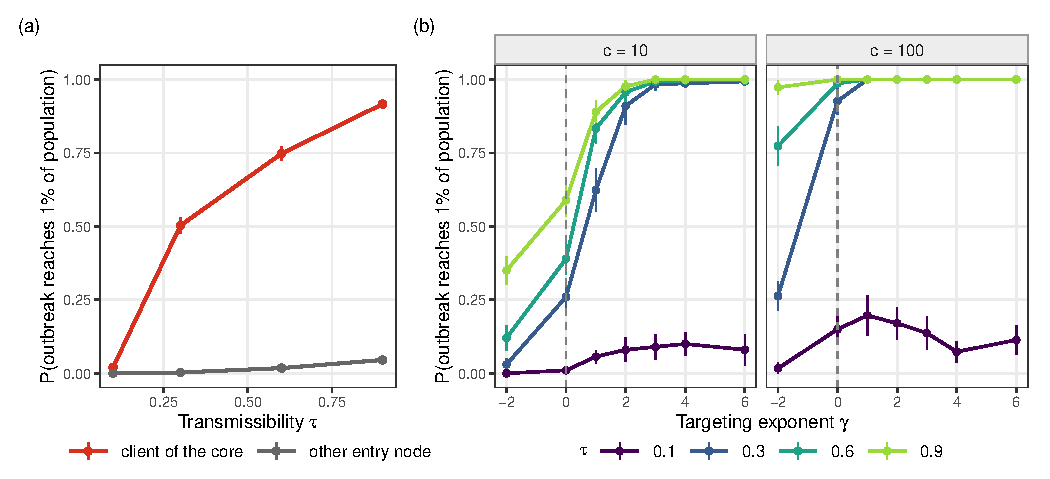
\includegraphics[width=0.9\textwidth]{fig5_core_network.pdf}
\caption{Core network ($5\times10^4$ per sex, 10 networks). (a) Probability that one
seeding event reaches 1\% of the population, for an entry node that is a
client and for other entry nodes. (b) The same under repeated forcing against $\gamma$.}
\end{figure}
\textbf{Numbers and analysis.} Single seeding at $\tau=0.1/0.3/0.6/0.9$: clients
2/50/75/92\%, other entry nodes 0/0.3/1.8/4.5\%. Repeated forcing ($\tau=0.3$, $c=10$):
0.03 ($\gamma=-2$), 0.26 ($\gamma=0$), 0.91 ($\gamma=2$), $\ge0.98$ ($\gamma\ge3$). Here targeting decides
\emph{whether} a large outbreak occurs. The core (about 25 sex workers shared
by clients) is small and loop-rich, so the tree-like theory does not describe
it; this structured case is the subject of the follow-up study.

%%%%%%%%%%%%%%%%%%%%%%%%%%%%%%%%%%%%%%%%%%%%%%%%%%%%%%%%%%%%%%%%%%%%%%
\section{Numerical methods}
%%%%%%%%%%%%%%%%%%%%%%%%%%%%%%%%%%%%%%%%%%%%%%%%%%%%%%%%%%%%%%%%%%%%%%
\begin{longtable}{p{3.2cm}p{11.8cm}}
\toprule Component & Settings \\ \midrule \endfirsthead
\toprule Component & Settings \\ \midrule \endhead
Transmission & $\rho=1/14$ per day ($r=0.069$); for a target $\tau$, $p=\tau r/[(1-r)(1-\tau)]$; runs to extinction. \\
Forcing profile & 17-week incidence curve normalized to a maximum of 1, constant within weeks; $\sum_t\alpha_t=48.4$. \\
Linear response & 100 networks per distribution, $5\times10^3$ per sex; 30 events per degree and network; $\tau\in\{0.2,0.4,0.6,0.8,0.9\}$. \\
Repeated forcing & 50 networks; 10 runs; $c\in\{10,50,200\}$, $\tau\in\{0.6,0.9\}$, $\gamma\in\{-2,-1.5,\dots,6\}$. \\
$\gamma^*$ on networks & 100 networks per law; $c=10^{0},10^{0.1},\dots,10^{3.5}$; $\gamma\in[-1,30]$ in steps of 0.05; curves flat to relative $10^{-9}$ are not identifiable. \\
Scaling & i.i.d.\ uncapped degrees; $n=10^2,\dots,10^6$ with 2000/1000/1000/500/200 samples; sums over distinct values; $\theta$ = slope of mean $\ln\mu$ against $\ln n$ for $n\ge10^3$. \\
Limit curve & sums to $k=10^6$ plus analytic tail integral; $1-e^{-y}$ as $-\mathrm{expm1}(-y)$; finite-$n$ grid step 0.005 ($\gamma<1$) and 0.01 above. \\
Generalization & $\eta\in\{0.5,1,1.5,2\}$ (scaling), $\{0.5,1,2\}$ (limits); caps 25, 50, 100, 400. \\
Major outbreaks & NB$(1.2,0.7)$ networks; 20 networks; major = $0.5\times$ theoretical size (minimum 100). \\
Core network & 10 networks, $5\times10^4$ per sex; 300 single seedings per entry-node type; 30 forced runs; large outbreak = 1000 cases. \\
\bottomrule
\end{longtable}

%%%%%%%%%%%%%%%%%%%%%%%%%%%%%%%%%%%%%%%%%%%%%%%%%%%%%%%%%%%%%%%%%%%%%%
\section{Validity, limitations and validation status}\label{sec:validation}
%%%%%%%%%%%%%%%%%%%%%%%%%%%%%%%%%%%%%%%%%%%%%%%%%%%%%%%%%%%%%%%%%%%%%%
\paragraph{Where the theory holds.} (1) Below threshold with $R\lesssim0.9$. (2) When the
attack fraction $C/(N_1+N_2)$ is small, so that clusters do not overlap; the
error reaches about 10\% under intense, highly transmissible forcing. (3) For
entry-node importances drawn independently, and, in the degree model, $a>3$.
(4) The transition results are asymptotic in $n$; real pools are in the
rounded regime below $n_c$. (5) The bound $\gamma^*\le\gamma_2$ and the small-$x$ law hold as
$n\to\infty$; finite pools need $x\gtrsim3/\sqrt n$ to be within 0.1 of the limit. (6) The
small-$x$ formula applies below an $(a,\eta)$-dependent value of $x$.

\paragraph{Limitations.} Static network; no clustering or loops except in the
core illustration, where the tree theory fails; entry-node status independent
of degree; survey under-sampling of very active people (partly addressed by
the core); expected burden optimized, not its median or the probability of a
large outbreak; hypothetical pathogen, so no claims about a specific epidemic.

%% Validation status table (report only).
\begin{longtable}{p{4.2cm}p{7.2cm}p{3.6cm}}
\toprule Result & Evidence & Status \\ \midrule \endfirsthead
\toprule Result & Evidence & Status \\ \midrule \endhead
Linear response $s(k)=Ak$ & 100-network ensembles, median $|z|<1$; $R\lesssim0.9$ & validated \\
$\Prob(\text{no secondary})$ & within 0.044 everywhere & validated \\
$I(\gamma)$ & $|z|<2$ in all combinations & validated \\
$C(\gamma)$, intermediate $\gamma^*$ & $|z|\lesssim2$ except intense, high-$\tau$ forcing ($-10\%$) & validated \\
$\gamma^*>0$, $I$ max at 0 & 30\,960 cases, no exception & validated \\
$\theta(\gamma)$ ($\eta=1$) & plateaus within 3\% & validated \\
$Y_2$ limit & $n=10^6$ within a few hundredths & validated \\
$K/x$ & limit vs $K/x$ at $x\ge10$ within 5\% & validated \\
Small-$x$ law (fitted) & $c_a\approx a-1$ within 13\% & superseded by Prop.~\ref{prop:smallx} \\
$\theta_\eta$, $\eta\ne1$ & $\eta=0.5,1,1.5,2$: kink moves with $\gamma_1=a-1-\eta$; plateaus $\eta/(a-1)$ within 4\% & validated \\
Small-$x$ leading order & $|\gamma^*_\infty-[\gamma_2-(a-1)/\log(1/x)]|\le0.07$ for $\eta\ge1$, $x\le10^{-4}$; slower for $\eta=0.5$ (0.22 at $10^{-4}$, 0.07 at $10^{-8}$ for $a=4$) & validated (asymptotic) \\
$K/x$ for $\eta\ne1$ & $x=10$: 0.082/0.080/0.173 vs exact 0.078/0.076/0.157 & validated \\
Cut-off crossover & ratios $\approx1$ for $n/n_c\lesssim0.05$, 0.25--0.5 at $n/n_c\approx1$, $\to0$ for $n\gg n_c$; 4 caps, 2 laws & validated \\
Major outbreaks & synthetic networks, $|z|<2.3$ for $\tau\ge0.5$ & validated (SM) \\
\bottomrule
\end{longtable}


\bibliographystyle{unsrt}
\bibliography{../references}
\end{document}
